\documentclass[10pt]{article}
\usepackage[english]{babel}
\usepackage[latin1]{inputenc}
\usepackage{subfigure}
\usepackage{epsfig}
\usepackage{amsmath,amssymb}
\parindent 0mm
\textwidth 16cm
\textheight 23cm
\oddsidemargin 0cm
\evensidemargin 0cm
\topmargin -10mm
\newcommand{\vect}[1]{{\bf{#1}}}
\newcommand{\svect}[1]{\boldsymbol{#1}}
\newcommand{\matr}[1]{\boldsymbol{#1}}


\begin{document}
\pagestyle{empty}
\begin{Large}
\begin{bf} 
T-61.5130 Machine Learning and Neural Networks\\ 
\end{bf}
\end{Large}
Karhunen, Hao Tele\\  
\\
\begin{large}
\begin{bf}
Exercise 4,  17.11.2011
\end{bf}
\end{large}
\begin{enumerate}

\item Construct an MLP network which is able to separate the two
  classes illustrated in Figure \ref{61}. Use two neurons both in the input
  and output layer and an arbitrary number of hidden layer
  neurons. The output of the network should be vector $\left[ 1,
  0\right]^T$ if the input vector belongs to class $\mathcal{C}_1$ and  $\left[ 0,
  1\right]^T$ if it belongs to class $\mathcal{C}_2$. Use nonlinear activation
  functions, namely McCulloch-Pitts model, for all the neurons and
  determine their weights by hand without using any specific learning
  algorithm.
\begin{itemize}
\item[(a)] What is the minimum amount of neurons in the hidden layer
  required for a perfect separation of the classes?
\item[(b)] What is the maximum amount of neurons in the hidden layer?
\end{itemize}

\begin{figure}[hbp]
\centering
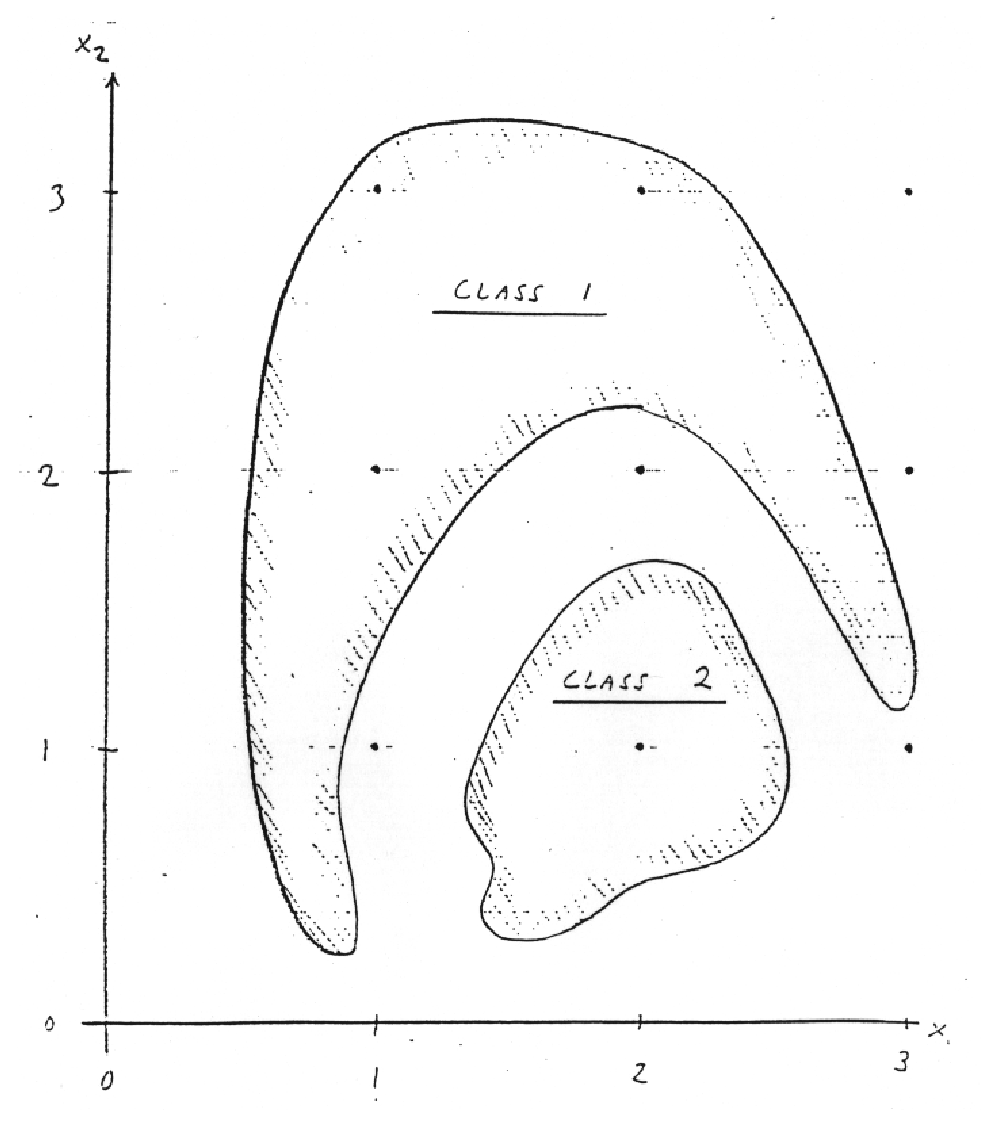
\includegraphics[width=7cm]{mlp_classification.ps}
\label{61}
\caption{Classes $\mathcal{C}_1$ and $\mathcal{C}_2$.}
\end{figure}

\vspace{2mm}

\item The function
\[
t(x) = x^2, \hspace{3mm} x \in \left[ 1, 2 \right]
\]
is approximated with a neural network. The activation functions of all
the neurons are linear functions of the input signals and a constant
bias term. The number of neurons and the network architecture can be
chosen freely. The approximation performance of the network is
measured with the following error function:
\[
\mathcal{E} = \int_{1}^2 \left[ t({\bf x})-y({\bf x}) \right]^2 d{\bf x}
\]
where $\vect{x}$ is the input vector of the network and $y(\vect{x})$ is the
corresponding response.
\begin{itemize}
\item[(a)] Construct a single-layer network which minimizes the error function.
\item[(b)] Does the approximation performance of the network improve if
  additional hidden layers are included?
\end{itemize}

\vspace{2mm}

\item (Matlab demo)

\end{enumerate}
\end{document}             % End of document.
